% CoRL 2026 Supplementary Material
% Companion to manuscript.tex
\documentclass[conference]{IEEEtran}
\usepackage{amsmath,amssymb,amsfonts}
\usepackage{graphicx}
\usepackage{textcomp}
\usepackage{xcolor}
\usepackage{url}
\usepackage{booktabs}
\usepackage{multirow}
\usepackage{subcaption}
\usepackage{caption}
\usepackage{placeins}
\usepackage{algorithm}
\usepackage{algorithmic}
\usepackage{hyperref}

\captionsetup{font=small,labelfont=bf,skip=4pt,justification=raggedright,singlelinecheck=false}
\captionsetup[subfigure]{font=footnotesize,labelfont=bf,skip=2pt,justification=raggedright,singlelinecheck=false}
\setlength{\textfloatsep}{8pt plus 1.0pt minus 2.0pt}
\setlength{\floatsep}{6pt plus 1.0pt minus 2.0pt}
\renewcommand{\arraystretch}{0.94}

\newcommand{\brier}{B_{\mathrm{soft}}}
\newcommand{\kl}{D_{\mathrm{KL}}}
\newcommand{\hmax}{H_{\max}}

% Make this an appendix-style numbering
\renewcommand{\thesection}{S\arabic{section}}
\renewcommand{\thetable}{S\arabic{table}}
\renewcommand{\thefigure}{S\arabic{figure}}
\renewcommand{\theequation}{S\arabic{equation}}

\begin{document}

\title{Supplementary Material:\\
Human-Aligned Sidewalk Accessibility Perception\\
Soft-Label Learning from 829 Mobility-Aid Users}
\maketitle

\noindent\emph{This document accompanies the main paper. Tables, figures, and equations are numbered with the prefix~S. References to numbered results in the main paper are written as ``main Table~X'' or ``main Fig.~X.''}

\tableofcontents
\vspace{1em}

\section{Full Per-Encoder Per-Aid Results}
\label{sec:supp_full_cv}

Tables~\ref{tab:supp_softkl_f1}, \ref{tab:supp_hardce_f1}, \ref{tab:supp_softkl_brier}, \ref{tab:supp_hardce_brier}, and \ref{tab:supp_ece} extend main Table~2 (ablation) and main Table~1 (Hard-CE encoder ranking) by reporting macro-F1, balanced accuracy, soft Brier score, and ECE per encoder and per aid for both training objectives. All numbers are 5-fold panorama-level CV with seed = 42, identical to the main paper. The bold cells highlight the best encoder per aid within each objective.

\begin{table*}[!t]
\caption{\textbf{Soft-KL: per-aid macro-F1.} Best per column in bold.}
\label{tab:supp_softkl_f1}
\centering\scriptsize
\setlength{\tabcolsep}{4pt}
\begin{tabular}{@{}lcccccc@{}}
\toprule
\textbf{Encoder} & \textbf{Cane} & \textbf{Walker} & \textbf{Scooter} & \textbf{Man.WC} & \textbf{Mot.WC} & \textbf{Mean} \\
\midrule
CLIP B/32      & 0.513 & 0.625 & 0.544 & 0.459 & 0.509 & 0.530 \\
CLIP B/16      & 0.414 & 0.542 & 0.537 & 0.532 & 0.469 & 0.499 \\
CLIP L/14      & 0.618 & 0.503 & 0.446 & \textbf{0.557} & 0.529 & 0.531 \\
DINOv2-base    & 0.493 & 0.510 & 0.470 & 0.408 & 0.599 & 0.496 \\
DINOv2-large   & \textbf{0.640} & \textbf{0.667} & \textbf{0.656} & 0.531 & 0.573 & \textbf{0.613} \\
SigLIP2-base   & 0.461 & 0.574 & 0.459 & 0.444 & 0.571 & 0.502 \\
SigLIP2-SO400M & 0.511 & 0.600 & 0.601 & 0.530 & \textbf{0.652} & 0.579 \\
ViT-B/16-sup   & 0.408 & 0.603 & 0.529 & 0.429 & 0.442 & 0.482 \\
\bottomrule
\end{tabular}
\end{table*}

\begin{table*}[!t]
\caption{\textbf{Hard-CE: per-aid macro-F1.} Best per column in bold.}
\label{tab:supp_hardce_f1}
\centering\scriptsize
\setlength{\tabcolsep}{4pt}
\begin{tabular}{@{}lcccccc@{}}
\toprule
\textbf{Encoder} & \textbf{Cane} & \textbf{Walker} & \textbf{Scooter} & \textbf{Man.WC} & \textbf{Mot.WC} & \textbf{Mean} \\
\midrule
CLIP B/32      & 0.453 & \textbf{0.761} & 0.558 & \textbf{0.675} & 0.639 & \textbf{0.617} \\
CLIP B/16      & 0.434 & 0.536 & 0.569 & 0.562 & 0.618 & 0.544 \\
CLIP L/14      & 0.453 & 0.707 & 0.698 & 0.523 & 0.597 & 0.595 \\
DINOv2-base    & 0.446 & 0.720 & 0.668 & 0.574 & \textbf{0.664} & 0.614 \\
DINOv2-large   & 0.489 & 0.675 & \textbf{0.746} & 0.502 & 0.652 & 0.613 \\
SigLIP2-base   & 0.458 & 0.700 & 0.587 & 0.572 & 0.664 & 0.596 \\
SigLIP2-SO400M & 0.453 & 0.669 & 0.519 & 0.483 & 0.652 & 0.555 \\
ViT-B/16-sup   & \textbf{0.513} & 0.682 & 0.606 & 0.553 & 0.509 & 0.573 \\
\bottomrule
\end{tabular}
\end{table*}

\begin{table*}[!t]
\caption{\textbf{Soft-KL: per-aid soft Brier score ($\downarrow$).} Lower is better (perfect calibration = 0). All values $<0.15$, vs.\ Hard-CE values $\geq 0.19$ in Table~\ref{tab:supp_hardce_brier}.}
\label{tab:supp_softkl_brier}
\centering\scriptsize
\setlength{\tabcolsep}{4pt}
\begin{tabular}{@{}lcccccc@{}}
\toprule
\textbf{Encoder} & \textbf{Cane} & \textbf{Walker} & \textbf{Scooter} & \textbf{Man.WC} & \textbf{Mot.WC} & \textbf{Mean} \\
\midrule
CLIP B/32      & 0.051 & 0.066 & 0.044 & 0.059 & 0.103 & 0.064 \\
CLIP B/16      & 0.059 & 0.085 & 0.048 & 0.070 & 0.139 & 0.080 \\
CLIP L/14      & 0.061 & 0.076 & 0.068 & 0.087 & 0.109 & 0.080 \\
DINOv2-base    & 0.072 & 0.079 & 0.063 & 0.082 & 0.102 & 0.080 \\
DINOv2-large   & 0.061 & 0.070 & 0.051 & 0.086 & 0.106 & 0.075 \\
SigLIP2-base   & 0.079 & 0.082 & 0.057 & 0.089 & 0.104 & 0.082 \\
SigLIP2-SO400M & 0.062 & 0.069 & 0.047 & 0.061 & 0.090 & 0.066 \\
ViT-B/16-sup   & 0.065 & 0.082 & 0.061 & 0.075 & 0.133 & 0.083 \\
\bottomrule
\end{tabular}
\end{table*}

\begin{table*}[!t]
\caption{\textbf{Hard-CE: per-aid soft Brier score ($\downarrow$).} Uniformly 3 to $4\times$ worse than Soft-KL across all (encoder, aid) cells.}
\label{tab:supp_hardce_brier}
\centering\scriptsize
\setlength{\tabcolsep}{4pt}
\begin{tabular}{@{}lcccccc@{}}
\toprule
\textbf{Encoder} & \textbf{Cane} & \textbf{Walker} & \textbf{Scooter} & \textbf{Man.WC} & \textbf{Mot.WC} & \textbf{Mean} \\
\midrule
CLIP B/32      & 0.229 & 0.213 & 0.234 & 0.243 & 0.234 & 0.231 \\
CLIP B/16      & 0.212 & 0.253 & 0.205 & 0.245 & 0.280 & 0.239 \\
CLIP L/14      & 0.200 & 0.221 & 0.239 & 0.249 & 0.240 & 0.230 \\
DINOv2-base    & 0.195 & 0.208 & 0.265 & 0.291 & 0.230 & 0.238 \\
DINOv2-large   & 0.211 & 0.235 & 0.242 & 0.304 & 0.272 & 0.253 \\
SigLIP2-base   & 0.197 & 0.231 & 0.245 & 0.235 & 0.234 & 0.228 \\
SigLIP2-SO400M & 0.208 & 0.265 & 0.244 & 0.270 & 0.293 & 0.256 \\
ViT-B/16-sup   & 0.218 & 0.288 & 0.268 & 0.259 & 0.336 & 0.274 \\
\bottomrule
\end{tabular}
\end{table*}

\begin{table*}[!t]
\caption{\textbf{Hard-label Expected Calibration Error (ECE, $\downarrow$).} ECE is computed against the majority hard label, not the full human vote distribution. It can therefore reward a model for being confidently aligned with the plurality class on images where humans are split. This explains cases where Hard-CE has lower ECE than Soft-KL despite being uniformly worse under soft Brier, which is the distributional metric consumed by the routing objective.}
\label{tab:supp_ece}
\centering\scriptsize
\setlength{\tabcolsep}{4pt}
\begin{tabular}{@{}lcc|cc@{}}
\toprule
& \multicolumn{2}{c|}{\textbf{Walking cane}} & \multicolumn{2}{c}{\textbf{Manual WC}} \\
\textbf{Encoder} & \textbf{Soft-KL} & \textbf{Hard-CE} & \textbf{Soft-KL} & \textbf{Hard-CE} \\
\midrule
CLIP B/32      & 0.270 & 0.179 & 0.202 & 0.238 \\
CLIP B/16      & 0.275 & 0.205 & 0.214 & 0.219 \\
CLIP L/14      & 0.223 & 0.166 & 0.258 & 0.269 \\
DINOv2-base    & 0.234 & 0.165 & 0.210 & 0.250 \\
DINOv2-large   & 0.243 & 0.185 & 0.274 & 0.303 \\
SigLIP2-base   & 0.193 & 0.192 & 0.262 & 0.225 \\
SigLIP2-SO400M & 0.277 & 0.183 & 0.239 & 0.272 \\
ViT-B/16-sup   & 0.209 & 0.194 & 0.262 & 0.291 \\
\bottomrule
\end{tabular}
\end{table*}

This table should be read as a diagnostic for argmax-style classification, not as the primary calibration claim. Soft-KL deliberately assigns probability mass to minority and ``unsure'' responses when the vote distribution is broad; hard-label ECE treats that behaviour as under-confidence if the argmax still matches the majority class. The routing planner, however, uses the probability magnitude $\hat{p}_\mathrm{yes}$ as an edge cost, so the operational calibration target is the full vote distribution. Soft Brier directly measures that distributional error, while ECE bins are also high-variance in this setting because each per-aid fold contains only about ten held-out images.

\FloatBarrier
\section{Routing Graph Edge-Score Diagnostics}
\label{sec:supp_edge_diag}

Table~\ref{tab:supp_edge_sources} reports the source of each edge score in the Pittsburgh routing graph. Table~\ref{tab:supp_edge_dist} summarises the resulting $\hat{p}_\mathrm{yes}$ distributions. The GSV-inferred scores produce a broad probability range rather than a constant prior, which is necessary for Dijkstra to trade distance against aid-specific accessibility.

\begin{table}[!t]
\caption{\textbf{Routing graph score coverage.} Edge records are fixed in the 2,618-edge Pittsburgh graph used for Monte Carlo routing.}
\label{tab:supp_edge_sources}
\centering\scriptsize
\setlength{\tabcolsep}{6pt}
\begin{tabular}{@{}lcc@{}}
\toprule
\textbf{Source} & \textbf{Edges} & \textbf{Share} \\
\midrule
Project Sidewalk labels & 1,057 & 40.4\% \\
GSV model inference & 1,344 & 51.3\% \\
Population prior fallback & 217 & 8.3\% \\
\bottomrule
\end{tabular}
\end{table}

\begin{table*}[!t]
\caption{\textbf{Per-aid edge-score distributions.} Values are over all 2,618 graph edge records after Project Sidewalk labels, GSV inference, and prior fallback are merged.}
\label{tab:supp_edge_dist}
\centering\scriptsize
\setlength{\tabcolsep}{5pt}
\begin{tabular}{@{}lcccccc@{}}
\toprule
\textbf{Aid} & \textbf{Mean} & \textbf{P10} & \textbf{P50} & \textbf{P90} & \textbf{\% $<0.50$} & \textbf{\% $\geq0.80$} \\
\midrule
Walking cane         & 0.668 & 0.376 & 0.698 & 0.920 & 13.8 & 24.7 \\
Walker               & 0.557 & 0.276 & 0.500 & 0.880 & 46.3 & 13.4 \\
Mobility scooter     & 0.524 & 0.245 & 0.530 & 0.850 & 44.6 & 13.6 \\
Manual wheelchair    & 0.479 & 0.243 & 0.500 & 0.820 & 49.5 & 13.4 \\
Motorized wheelchair & 0.482 & 0.222 & 0.466 & 0.840 & 52.6 & 13.4 \\
\bottomrule
\end{tabular}
\end{table*}

\textbf{DINOv2 feature-support diagnostic for extrapolation.} The routing graph applies the 52-view probe to additional Pittsburgh GSV views, so this step is a transfer assumption rather than a direct calibration test. To quantify visual support in the same representation used by the routing probe, we embedded the 55 local audit images available on disk and 437 labelled GSV images from Pittsburgh, Detroit, Zurich, and Taipei with frozen DINOv2-large. Distances are nearest-audit cosine distances in the L2-normalised feature space; the audit leave-one-out distribution provides an in-support reference scale. Table~\ref{tab:supp_visual_support} shows that Pittsburgh routing-style images lie close to the audit support under DINOv2 (12.3\% above the audit P90, near the 10\% leave-one-out reference), while Taipei is entirely outside this support, matching the near-chance Taipei transfer result in main Table~5. We therefore treat routing inference as a supported Pittsburgh map-prior demonstration, not as evidence that the 52-view Brier calibration is preserved globally. A deployed AV system should combine this prior with live onboard verification or an OOD gate.

\begin{table*}[!t]
\caption{\textbf{DINOv2-large feature-support diagnostic.} Nearest-audit cosine distance in the same frozen feature space used by the Soft-KL routing probe. Higher values mean farther from the 52-view audit support. ``Above audit P90'' is the fraction of external images farther than the 90th percentile of audit leave-one-out distances.}
\label{tab:supp_visual_support}
\centering\scriptsize
\setlength{\tabcolsep}{5pt}
\begin{tabular}{@{}lcccccc@{}}
\toprule
\textbf{Group} & \textbf{n} & \textbf{Mean} & \textbf{P25} & \textbf{P50} & \textbf{P90} & \textbf{Above audit P90} \\
\midrule
Audit leave-one-out & 55  & 0.428 & 0.347 & 0.408 & 0.610 & 10.0\% \\
Detroit             & 91  & 0.428 & 0.377 & 0.407 & 0.530 & 3.3\% \\
Pittsburgh          & 162 & 0.485 & 0.413 & 0.461 & 0.625 & 12.3\% \\
Taipei              & 95  & 0.768 & 0.740 & 0.773 & 0.819 & 100.0\% \\
Zurich              & 89  & 0.796 & 0.753 & 0.804 & 0.868 & 98.9\% \\
\bottomrule
\end{tabular}
\end{table*}

\FloatBarrier
\section[Barrier-Cost Pareto Sweep]{Pareto Sweep over Barrier-Cost $\beta_c$}
\label{sec:supp_pareto}

Table~\ref{tab:supp_pareto} reports the per-aid Pareto sweep over $\beta_c \in \{1,2,4,8,16\}$ on the canonical OD pair, the data underlying our $\beta_c = 8$ choice in main Section~6. Figure~\ref{fig:supp_pareto} visualises the same sweep averaged across aids. Table~\ref{tab:supp_beta_mc} reports the corresponding Monte Carlo sensitivity over 10,000 OD pairs. The Monte Carlo sweep confirms that the routing effect is not an artifact of the canonical pair: the improvement rate remains positive across all tested $\beta_c$, while distance overhead grows smoothly as accessibility is weighted more strongly.

\begin{table*}[!t]
\caption{\textbf{Barrier-cost sweep on the canonical OD pair.} Each cell shows ($\Delta\bar{p}_\mathrm{yes}$, $\Delta\ell$ \%). Bold marks the chosen operating point.}
\label{tab:supp_pareto}
\centering\scriptsize
\setlength{\tabcolsep}{4pt}
\begin{tabular}{@{}lccccc@{}}
\toprule
$\beta_c$ & \textbf{Cane} & \textbf{Walker} & \textbf{Scooter} & \textbf{Man.WC} & \textbf{Mot.WC} \\
\midrule
 1 & (0.029, 0.6) & (0.000, 0.0) & (0.000, 0.0) & (0.000, 0.0) & (0.000, 0.0) \\
 2 & (0.029, 0.6) & (0.026, 0.6) & (0.000, 0.0) & (0.000, 0.0) & (0.000, 0.0) \\
 4 & (0.145, 17.8) & (0.144, 24.8) & (0.140, 17.8) & (0.130, 17.8) & (0.133, 17.8) \\
\textbf{8} & \textbf{(0.155, 24.8)} & \textbf{(0.144, 24.8)} & \textbf{(0.140, 17.8)} & \textbf{(0.134, 19.3)} & \textbf{(0.146, 24.8)} \\
16 & (0.155, 24.8) & (0.144, 24.8) & (0.146, 24.8) & (0.140, 24.8) & (0.146, 24.8) \\
\bottomrule
\end{tabular}
\end{table*}

\begin{figure}[!t]
\centering
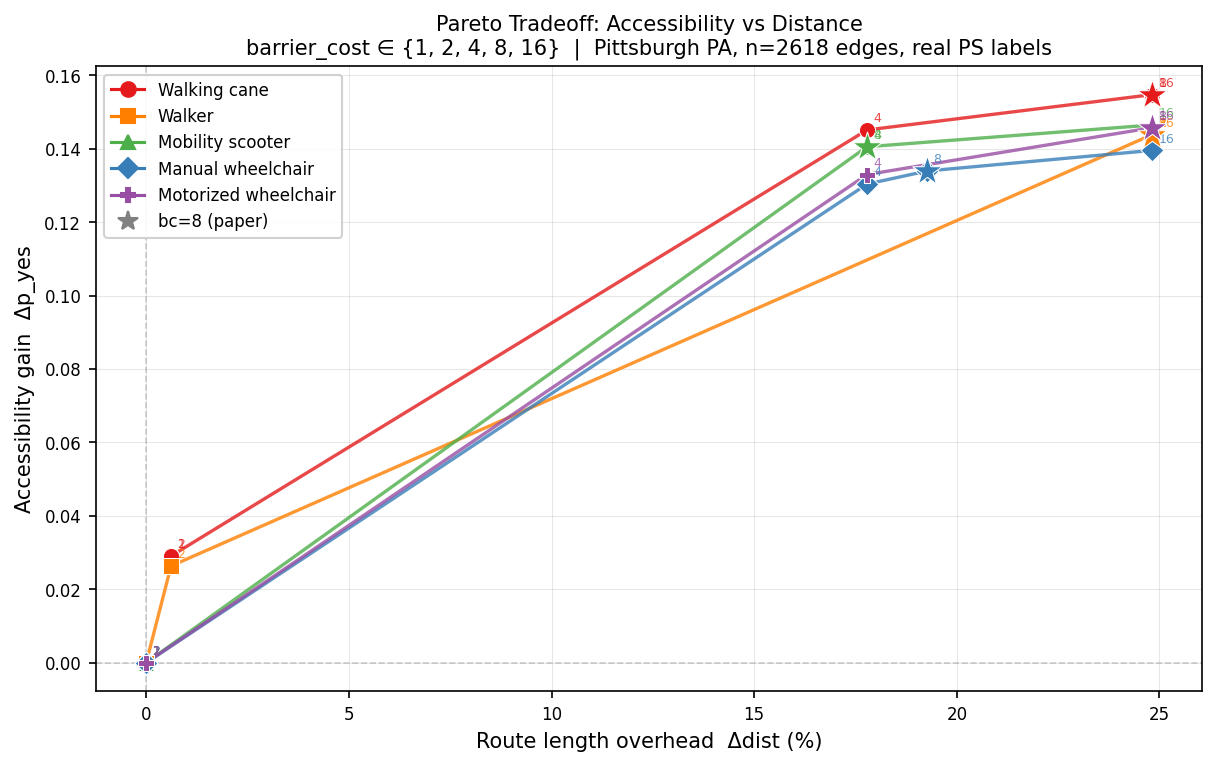
\includegraphics[width=\linewidth]{images/pareto_barrier_cost.png}
\caption{Pareto curve for $\beta_c \in \{1,2,4,8,16\}$. The accessibility gain saturates past $\beta_c=8$, justifying that as our operating point. Plot is averaged across the five mobility aids.}
\label{fig:supp_pareto}
\end{figure}

\begin{table*}[!t]
\caption{\textbf{Monte Carlo sensitivity to barrier cost $\beta_c$.} Each row averages over the five mobility aids and 10,000 Pittsburgh OD pairs. The operating point $\beta_c=8$ achieves most of the accessibility gain before the distance overhead begins to saturate.}
\label{tab:supp_beta_mc}
\centering\scriptsize
\setlength{\tabcolsep}{5pt}
\begin{tabular}{@{}lccccc@{}}
\toprule
$\beta_c$ & \textbf{Mean \% improved} & \textbf{Mean $\Delta\bar{p}_\mathrm{yes}$} & \textbf{Mean $\Delta\ell$ \%} & \textbf{Median $\Delta\ell$ \%} & \textbf{Improvement range} \\
\midrule
1  & 74.1 & 0.0575 & 1.98 & 1.18 & 68.9--77.1 \\
2  & 82.4 & 0.0718 & 3.62 & 2.41 & 78.1--86.2 \\
4  & 87.0 & 0.0851 & 6.06 & 4.16 & 83.8--89.5 \\
\textbf{8}  & \textbf{89.7} & \textbf{0.0968} & \textbf{8.76} & \textbf{5.90} & \textbf{87.8--91.0} \\
16 & 91.3 & 0.1054 & 11.28 & 7.91 & 90.3--92.0 \\
\bottomrule
\end{tabular}
\end{table*}

\FloatBarrier
\section{Full Monte Carlo Routing Distribution (10{,}000 OD pairs)}
\label{sec:supp_mc}

Table~\ref{tab:supp_mc_full} reports the distributional summary of the 10{,}000-pair Monte Carlo evaluation underlying main Table~6, and Figure~\ref{fig:supp_mc_box} shows the corresponding per-aid gain distributions. Distance overhead is right-skewed: the median overhead is lower than the mean for all aids, indicating that a subset of trips accounts for the longest detours. Note: $\Delta\bar{p}_\mathrm{yes}$ measures the \emph{model-predicted} passability gain---the same DINOv2-large Soft-KL probe scores both the standard and risk-aware routes. This is an offline planner-facing evaluation; onboard sensors would verify the curbside scene before the door opens.

\begin{table*}[!t]
\caption{\textbf{Full Monte Carlo distribution (10{,}000 OD pairs).} P25, P50, P75 of $\Delta\bar{p}_\mathrm{yes}$, plus mean/median distance overhead and the fraction of pairs improved. Pittsburgh OSM graph, $\beta_c=8$, seed=42, min separation 200~m.}
\label{tab:supp_mc_full}
\centering\scriptsize
\setlength{\tabcolsep}{3pt}
\begin{tabular}{@{}lcccccccc@{}}
\toprule
\textbf{Aid} & \multicolumn{3}{c}{$\Delta\bar{p}_\mathrm{yes}$} & \multicolumn{2}{c}{$\Delta\ell$ \%} & \textbf{\% impr.} & $\bar{p}_\mathrm{yes}^\mathrm{std}$ & $\bar{p}_\mathrm{yes}^\mathrm{acc}$ \\
\cmidrule(lr){2-4} \cmidrule(lr){5-6}
& P25 & P50 & P75 & Mean & Median & & & \\
\midrule
Walking cane         & 0.027 & 0.055 & 0.090 & 7.43 & 4.81 & 87.8 & 0.710 & 0.775 \\
Walker               & 0.036 & 0.074 & 0.116 & 8.20 & 5.34 & 88.2 & 0.607 & 0.688 \\
Mobility scooter     & 0.050 & 0.096 & 0.145 & 8.59 & 5.65 & 91.0 & 0.561 & 0.663 \\
Manual wheelchair    & 0.060 & 0.112 & 0.172 & 9.76 & 6.80 & 90.9 & 0.512 & 0.632 \\
Motorized wheelchair & 0.059 & 0.110 & 0.164 & 9.82 & 6.88 & 90.8 & 0.520 & 0.636 \\
\bottomrule
\end{tabular}
\end{table*}

\begin{figure}[!t]
\centering
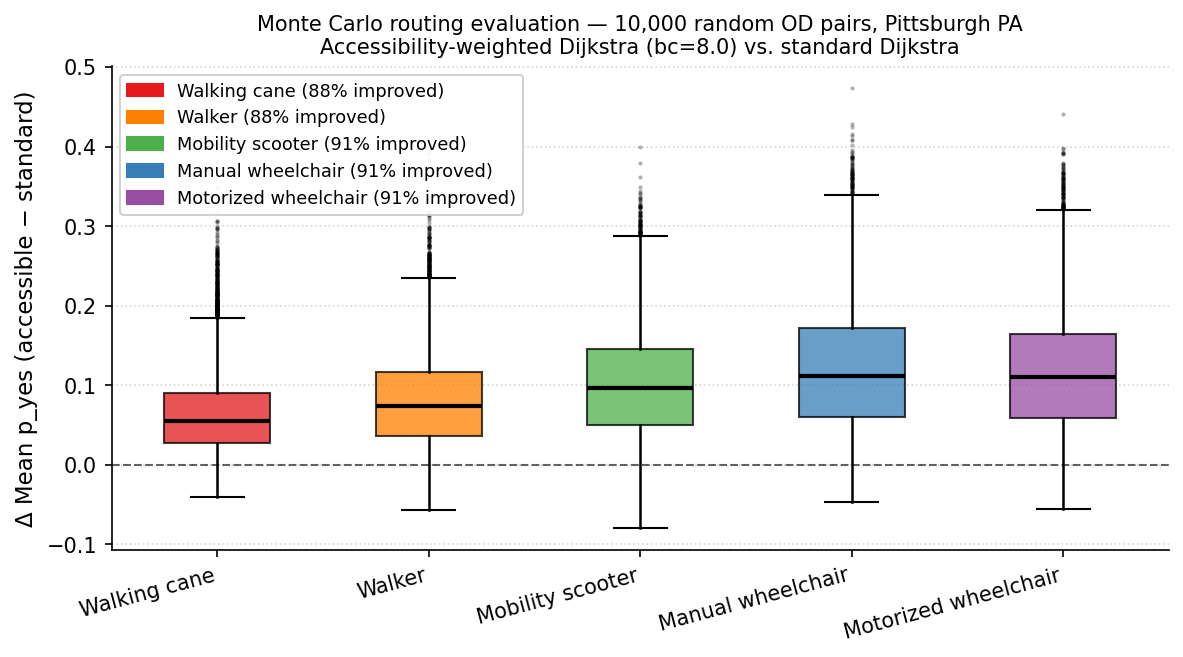
\includegraphics[width=\linewidth]{images/monte_carlo_boxplot.png}
\caption{Boxplot of per-aid $\Delta\bar{p}_\mathrm{yes}$ on 10{,}000 random OD pairs. All five aids show positive median improvement; the IQR confirms the rerouting benefit is widespread, not driven by outliers.}
\label{fig:supp_mc_box}
\end{figure}

\FloatBarrier
\section{Per-Aid OD-Pair Routing Visualisations}
\label{sec:supp_routes}

Figure~\ref{fig:supp_routes_grid} displays the per-aid accessible routes on the same OD pair as main Fig.~10, separately rendered to make each aid's routing geometry legible.

\begin{figure*}[!t]
\centering
\begin{subfigure}[t]{0.32\textwidth}
\centering\vspace{0pt}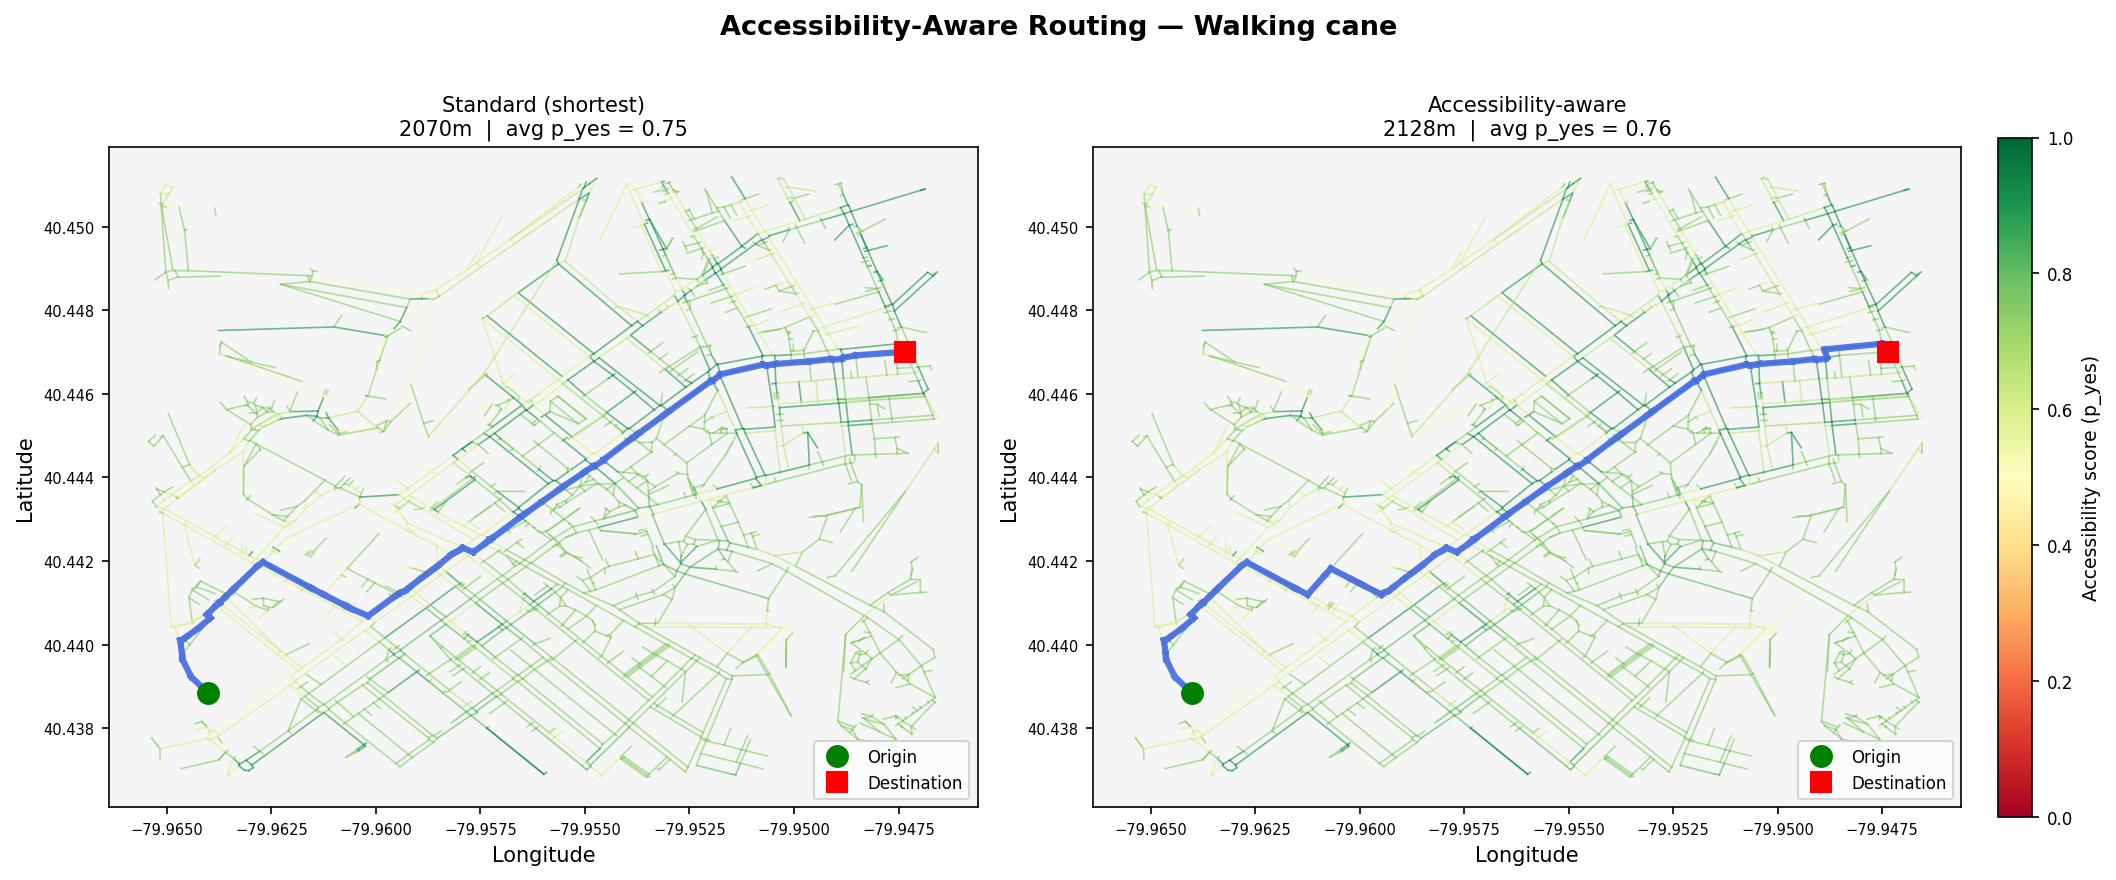
\includegraphics[width=\linewidth]{images/route_walking_cane.png}
\caption{Walking cane: $\bar{p}_\mathrm{yes} = 0.76$, $+2.8\%$ dist.}
\end{subfigure}
\hfill
\begin{subfigure}[t]{0.32\textwidth}
\centering\vspace{0pt}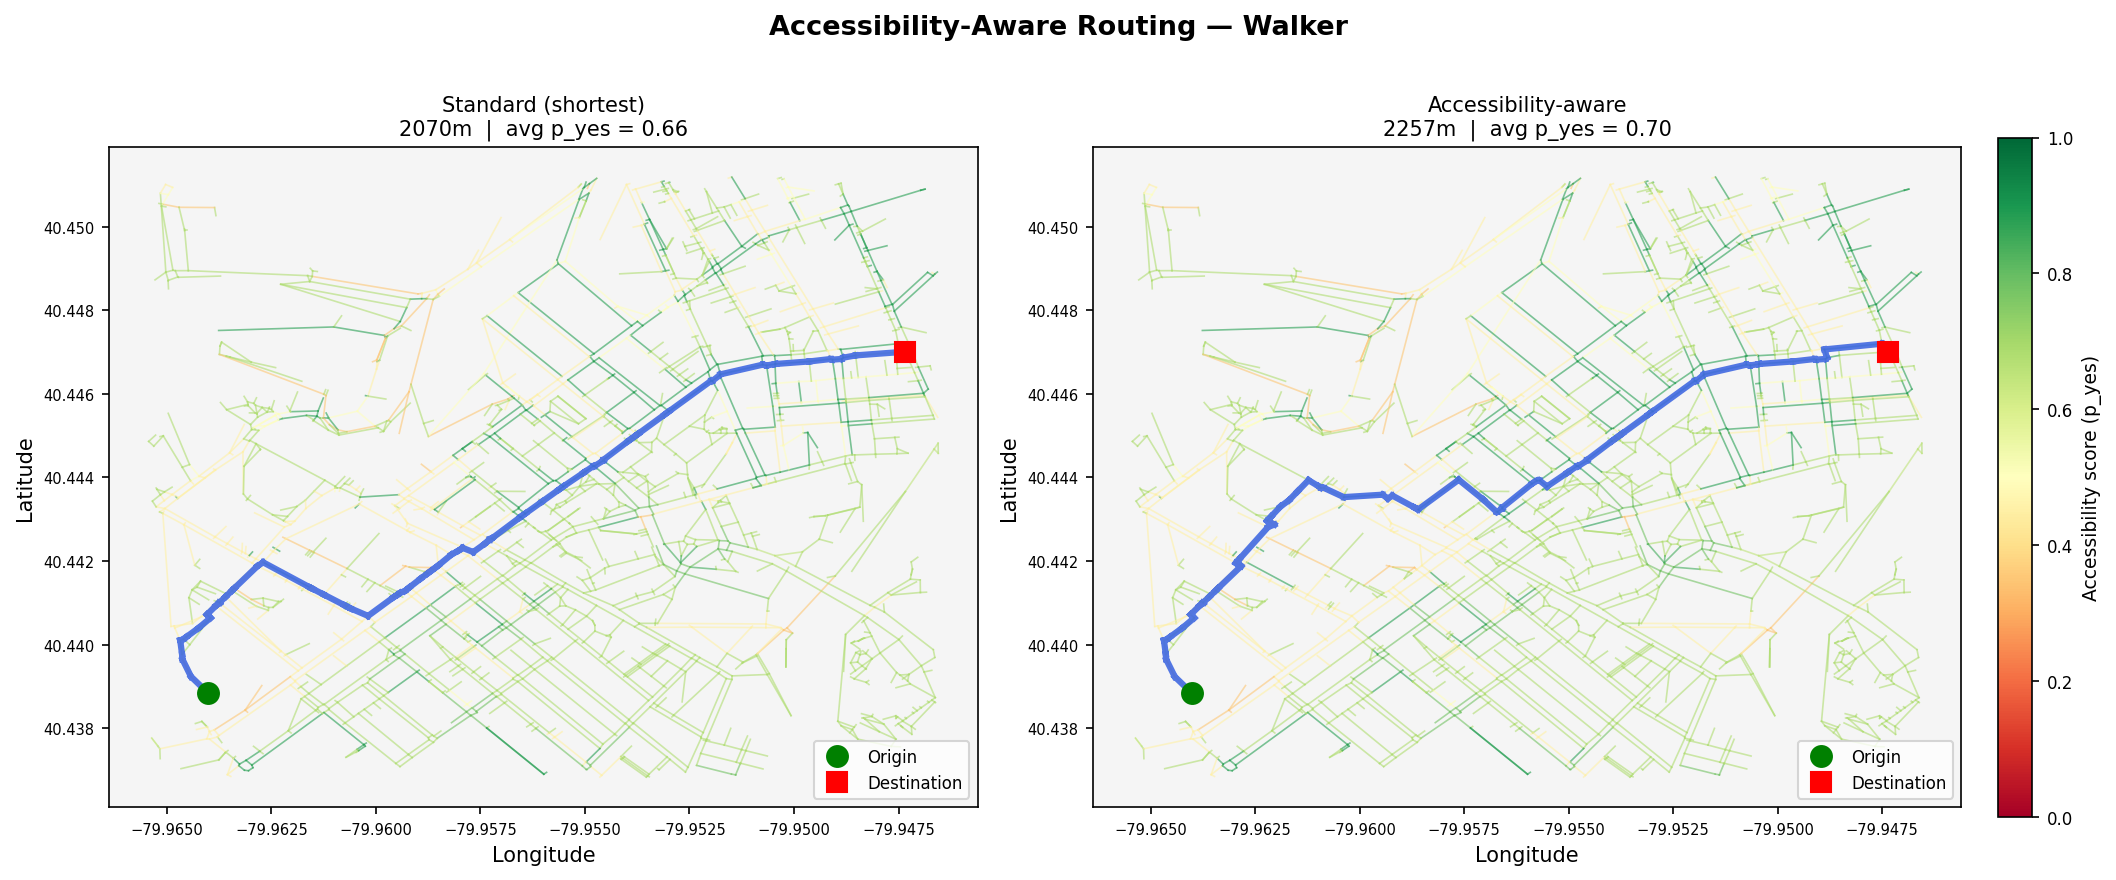
\includegraphics[width=\linewidth]{images/route_walker.png}
\caption{Walker: $\bar{p}_\mathrm{yes} = 0.70$, $+9.0\%$ dist.}
\end{subfigure}
\hfill
\begin{subfigure}[t]{0.32\textwidth}
\centering\vspace{0pt}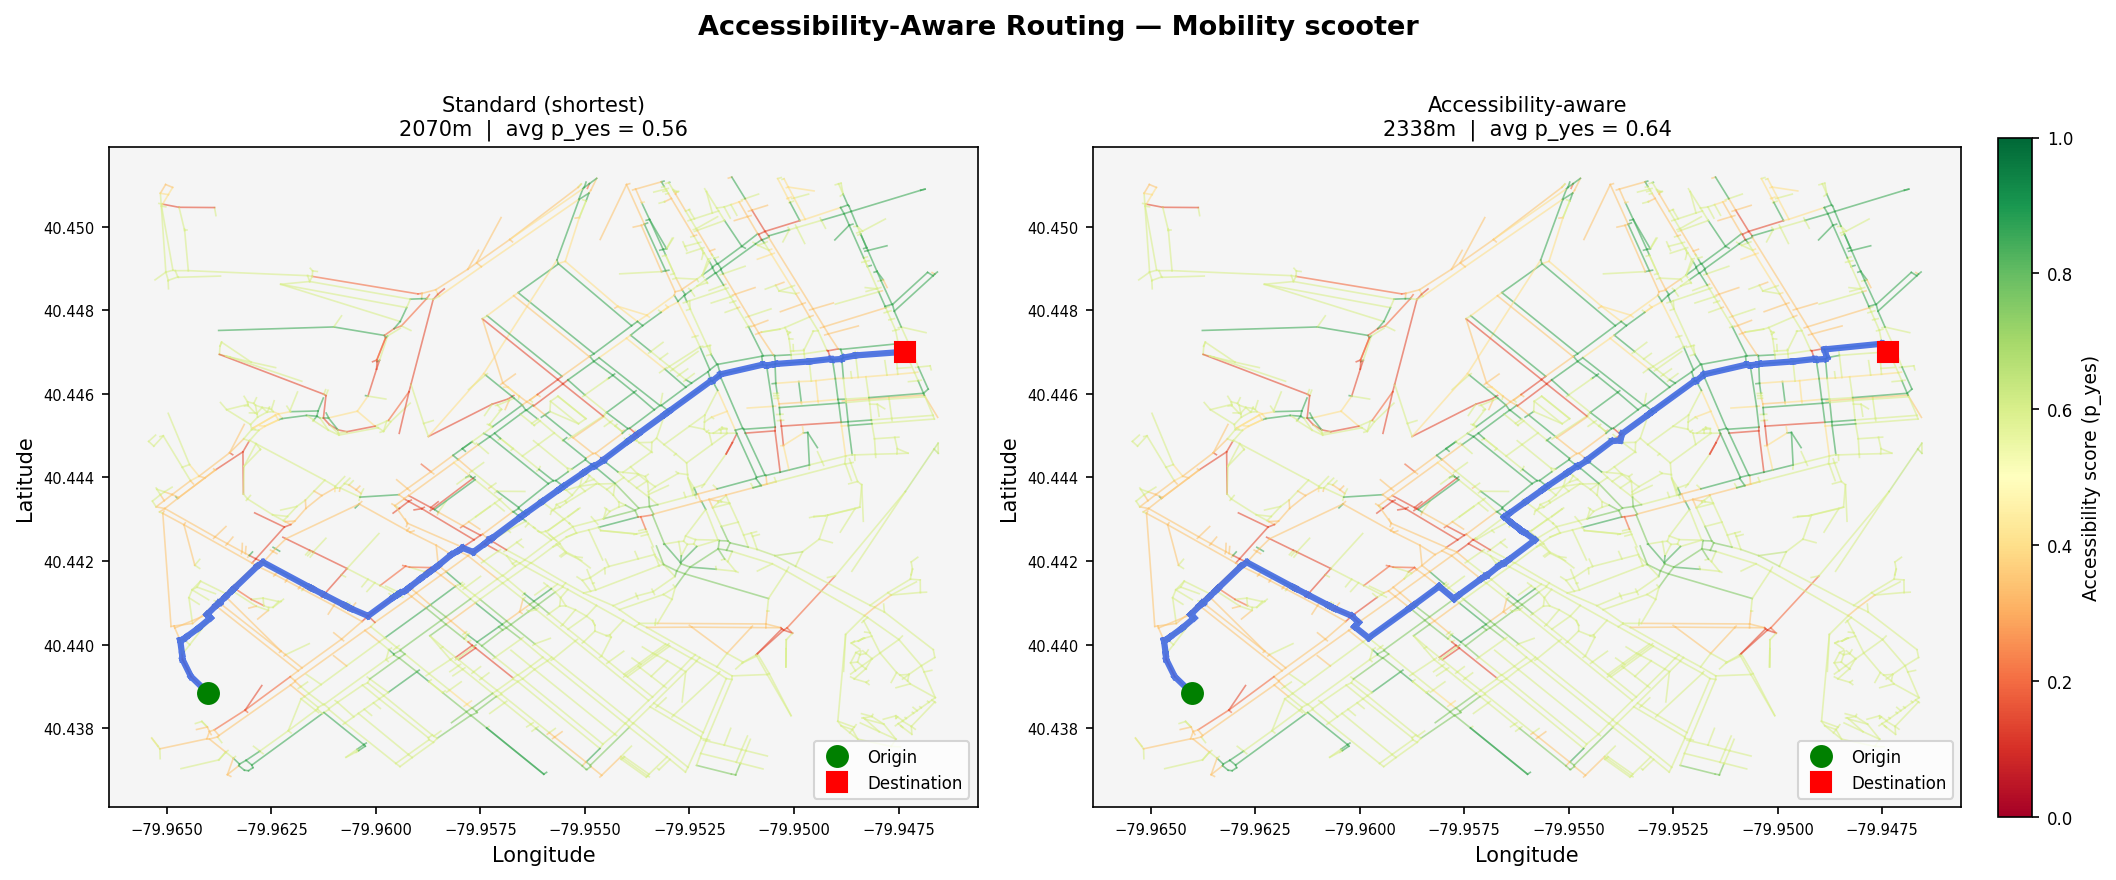
\includegraphics[width=\linewidth]{images/route_mobility_scooter.png}
\caption{Mobility scooter: $\bar{p}_\mathrm{yes} = 0.64$, $+12.9\%$ dist.}
\end{subfigure}\\[0.5em]
\hfill
\begin{subfigure}[t]{0.32\textwidth}
\centering\vspace{0pt}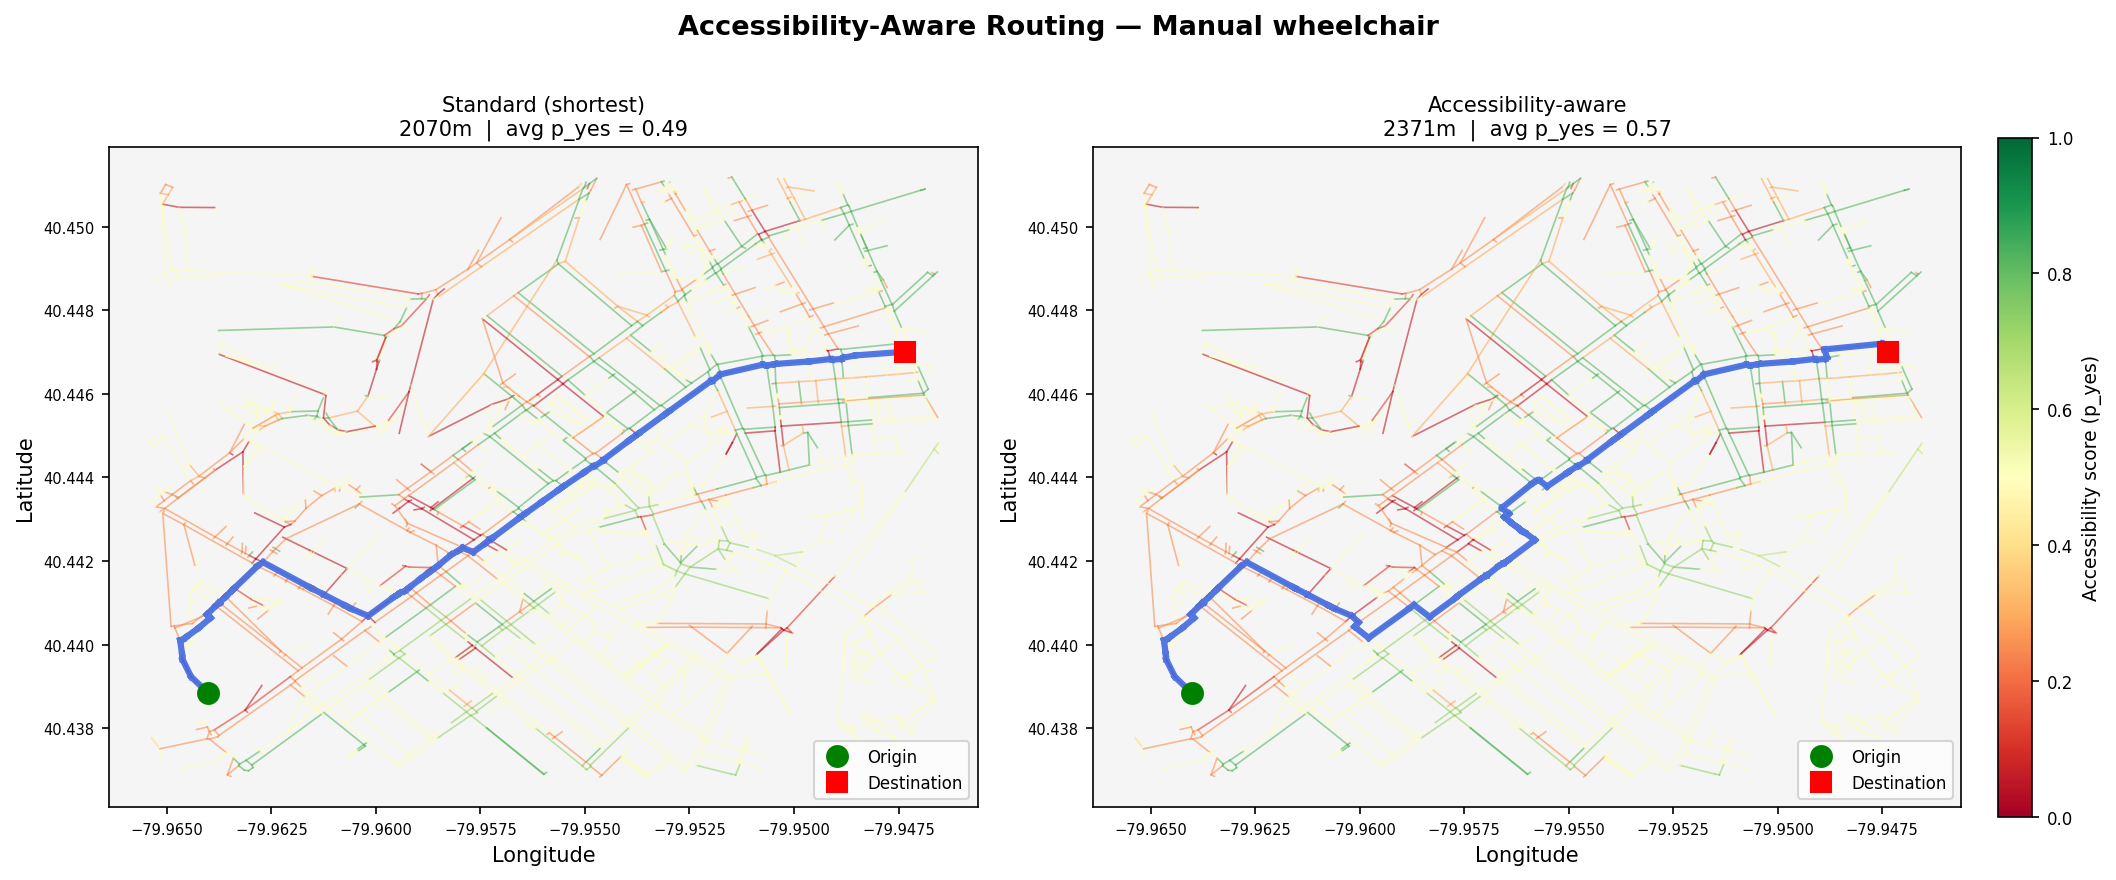
\includegraphics[width=\linewidth]{images/route_manual_wheelchair.png}
\caption{Manual wheelchair: $\bar{p}_\mathrm{yes} = 0.57$, $+14.5\%$ dist.}
\end{subfigure}
\hfill
\begin{subfigure}[t]{0.32\textwidth}
\centering\vspace{0pt}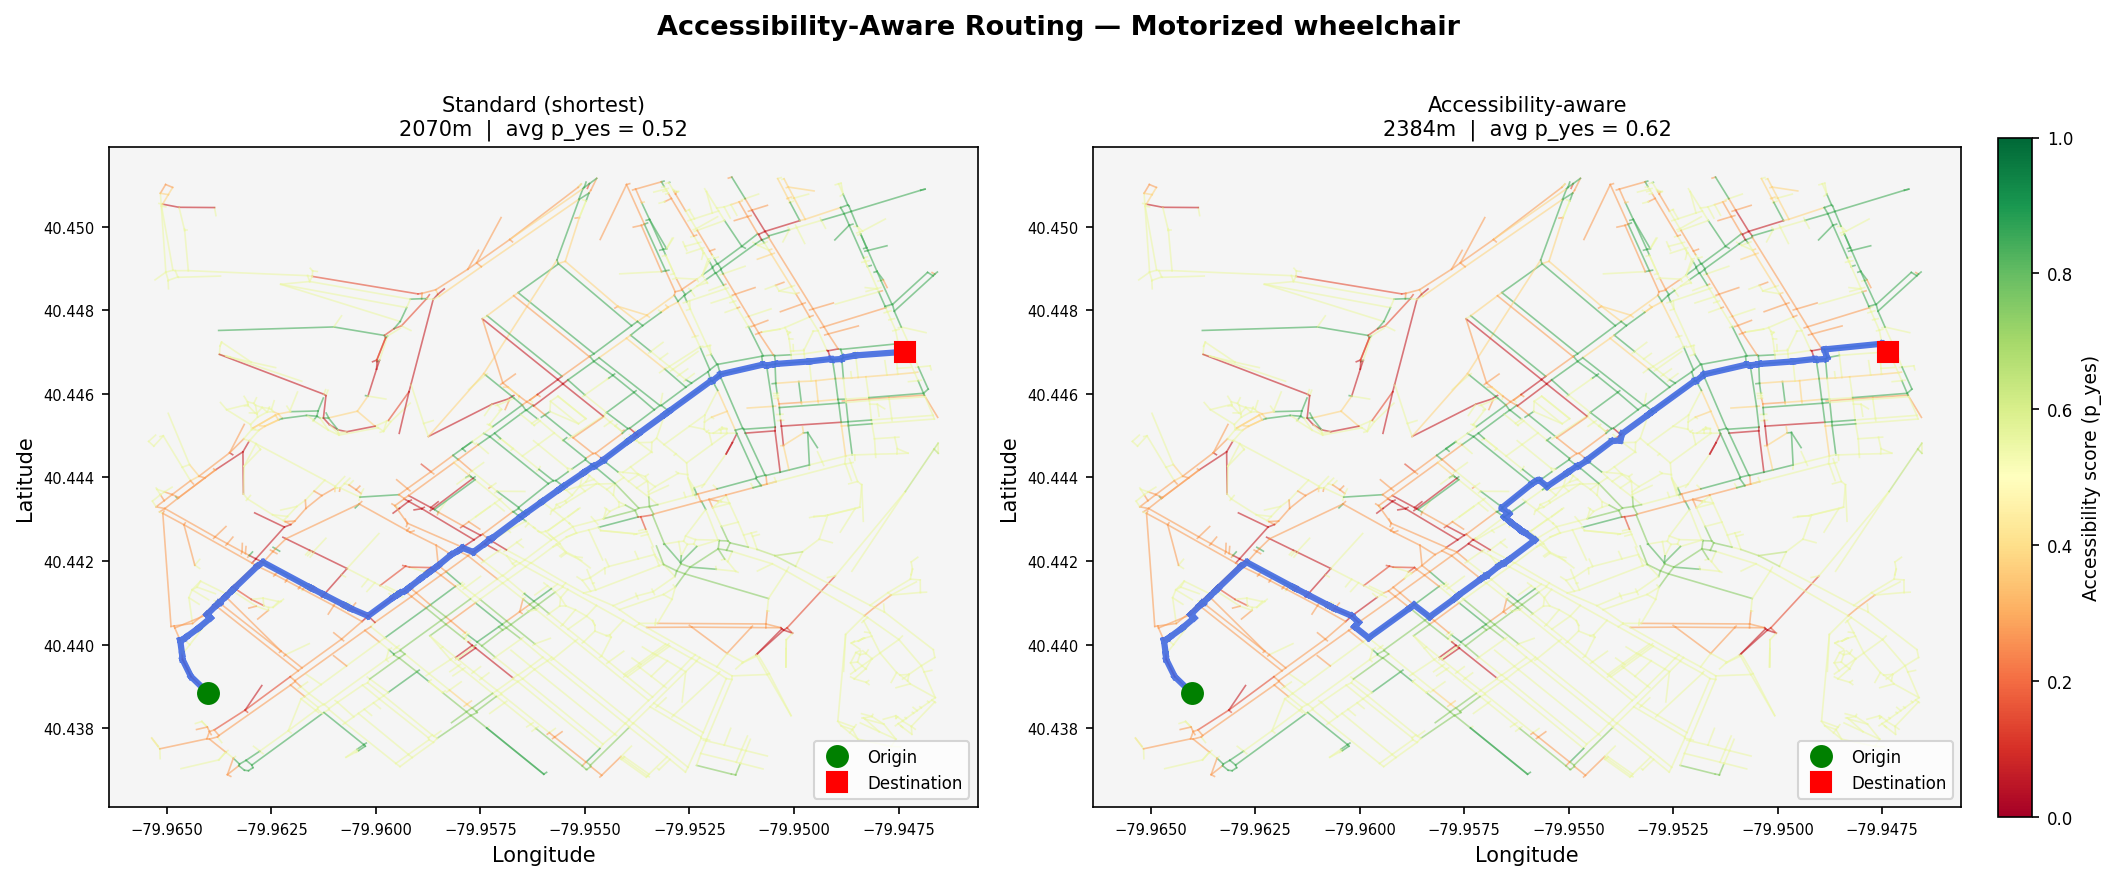
\includegraphics[width=\linewidth]{images/route_motorized_wheelchair.png}
\caption{Motorized wheelchair: $\bar{p}_\mathrm{yes} = 0.62$, $+15.1\%$ dist.}
\end{subfigure}
\hfill
\caption{\textbf{Per-aid accessible routes (canonical OD pair, $\beta_c=8$).} The five panels reveal that the optimal accessible path is aid-specific: walking-cane and walker (top, easier aids) take the most efficient detour; manual and motorized wheelchairs (bottom) prefer further-removed but smoother corridors.}
\label{fig:supp_routes_grid}
\end{figure*}

\FloatBarrier
\section{ORS Comparison Details}
\label{sec:supp_ors}

We queried the OpenRouteService public API \texttt{/v2/directions/wheelchair} endpoint between 2026-05-12 and 2026-05-14 for 50 random Pittsburgh OD pairs sampled from the same graph used in our Monte Carlo evaluation. ORS returned a successful route for 40 of 50 queries (80\%); the 10 failures (20\%) returned HTTP 400 with the error message \texttt{"Could not find routable point within radius."} Table~\ref{tab:supp_ors_full} reports the full per-aid comparison with both the standard Dijkstra and our accessibility-aware Dijkstra, including the absolute improvement margins.

\begin{table*}[!t]
\caption{\textbf{ORS wheelchair-profile comparison.} 40 routable OD pairs out of 50. ``Std.\ vs.\ ORS'' = gain ORS achieves over plain Dijkstra; ``Ours vs.\ ORS'' = our additional gain on top of ORS. Our method beats ORS on every aid by 0.033 to 0.046.}
\label{tab:supp_ors_full}
\centering\scriptsize
\setlength{\tabcolsep}{3.5pt}
\begin{tabular}{@{}lccccc@{}}
\toprule
\textbf{Aid} & \textbf{Std.} & \textbf{ORS} & \textbf{Ours} & \textbf{ORS$-$Std.} & \textbf{Ours$-$ORS} \\
\midrule
Walking cane         & 0.704 & 0.712 & 0.748 & $+0.009$ & $\mathbf{+0.036}$ \\
Walker               & 0.623 & 0.634 & 0.668 & $+0.011$ & $\mathbf{+0.034}$ \\
Mobility scooter     & 0.573 & 0.585 & 0.625 & $+0.012$ & $\mathbf{+0.040}$ \\
Manual wheelchair    & 0.505 & 0.519 & 0.566 & $+0.013$ & $\mathbf{+0.047}$ \\
Motorized wheelchair & 0.532 & 0.545 & 0.590 & $+0.013$ & $\mathbf{+0.045}$ \\
\midrule
\textit{Mean}        & 0.587 & 0.599 & 0.639 & $+0.012$ & $\mathbf{+0.040}$ \\
\bottomrule
\end{tabular}
\end{table*}

\FloatBarrier
\section{Hard-CE vs Soft-KL Routing Cross-Evaluation}
\label{sec:supp_hardce_routing}

Table~\ref{tab:supp_crosseval} reports the full cross-evaluation results for the canonical Pittsburgh OD pair (Forbes/Murray corridor). For each aid, we run accessibility-weighted Dijkstra separately under Soft-KL and Hard-CE DINOv2-large edge scores ($\beta_c = 8$), then evaluate both routes using the calibrated Soft-KL $\hat{p}_\mathrm{yes}$ metric. The gap column (Soft-KL route minus Hard-CE route, evaluated by Soft-KL) is positive for all five aids, confirming that miscalibrated edge scores produce suboptimal route choices. Hard-CE also inflates its self-assessed route quality (``HCE by HCE'') by +0.055 to +0.085, masking the true calibrated shortfall.

\begin{table}[!t]
\caption{\textbf{Hard-CE vs Soft-KL routing cross-evaluation on the canonical OD pair.} All $\hat{p}_\mathrm{yes}$ values evaluated by calibrated Soft-KL metric (ground truth), except the last column which shows Hard-CE's own (inflated) self-assessment. Gap = Soft-KL route minus Hard-CE route by calibrated metric. HCE routes are 430--436m overhead vs 412--575m for Soft-KL routes; despite being shorter, they are consistently less accessible.}
\label{tab:supp_crosseval}
\centering\small
\setlength{\tabcolsep}{4pt}
\begin{tabular}{@{}lcccccc@{}}
\toprule
\textbf{Aid} & \textbf{Std} & \textbf{SKL} & \textbf{HCE} & \textbf{Gap} & \textbf{HCE} & \textbf{HCE} \\
             & \textbf{(calibrated)} & \textbf{route} & \textbf{route} & \textbf{(SKL$-$HCE)} & \textbf{self-report} & \textbf{overestimate} \\
\midrule
Walking cane         & 0.516 & 0.671 & 0.657 & $+0.014$ & 0.721 & $+0.064$ \\
Walker               & 0.486 & 0.630 & 0.600 & $+0.030$ & 0.684 & $+0.085$ \\
Mobility scooter     & 0.459 & 0.600 & 0.587 & $+0.013$ & 0.675 & $+0.089$ \\
Manual wheelchair    & 0.442 & 0.576 & 0.561 & $+0.015$ & 0.660 & $+0.099$ \\
Motorized wheelchair & 0.446 & 0.592 & 0.572 & $+0.020$ & 0.625 & $+0.053$ \\
\bottomrule
\end{tabular}
\end{table}

\FloatBarrier
\section{Prompt-Sensitivity Per-Aid Decomposition}
\label{sec:supp_prompts}

Main Table~4 reports macro-F1 averaged over the five aids. Table~\ref{tab:supp_prompts_full} additionally reports balanced accuracy and per-prompt parse-failure counts. Across the 9 (model, prompt) combinations, only the CoT prompt on Qwen2.5-VL-7B incurred any parse failures (2 of 260 responses lacked a parseable label), confirming that prompt-engineering effects do not reduce to format-compliance differences.

\begin{table*}[!t]
\caption{\textbf{Full prompt-sensitivity matrix.} Three prompts (Direct / Descriptive / CoT) $\times$ three VLMs. Best per model in bold. Parse failures = number of responses (out of 260) lacking a parseable ternary label.}
\label{tab:supp_prompts_full}
\centering\scriptsize
\setlength{\tabcolsep}{5pt}
\begin{tabular}{@{}llccc@{}}
\toprule
\textbf{Model} & \textbf{Variant} & \textbf{F1} & \textbf{Bal.Acc} & \textbf{Parse fail} \\
\midrule
\multirow{3}{*}{Qwen3-VL-8B}   & Direct      & 0.513 & 0.532 & 0 \\
                                & \textbf{Descriptive} & \textbf{0.576} & \textbf{0.633} & 0 \\
                                & CoT         & 0.547 & 0.563 & 0 \\
\midrule
\multirow{3}{*}{LLaVA-1.5-7B}  & Direct      & 0.488 & 0.520 & 0 \\
                                & Descriptive & 0.430 & 0.514 & 0 \\
                                & \textbf{CoT}         & \textbf{0.542} & \textbf{0.563} & 0 \\
\midrule
\multirow{3}{*}{Qwen2.5-VL-7B} & \textbf{Direct}      & \textbf{0.442} & 0.610 & 0 \\
                                & Descriptive & 0.412 & 0.596 & 0 \\
                                & CoT         & 0.479 & \textbf{0.622} & 2 \\
\bottomrule
\end{tabular}
\end{table*}

\FloatBarrier
\section{Algorithms}
\label{sec:supp_algo}

\subsection{Soft-KL Probe Training}

\begin{algorithm}[!t]
\caption{Soft-KL training of a per-aid linear probe}
\label{alg:softkl}
\begin{algorithmic}[1]
\REQUIRE Frozen encoder $E$, training images $\{x_i\}_{i=1}^N$, vote distributions $\{\mathbf{y}_{i,a}\}$ for $a \in \mathrm{Aids}$
\STATE Pre-compute $\mathbf{f}_i = E(x_i)/\|E(x_i)\|_2$ once per image
\STATE Initialise $W_a, b_a$ from $\mathcal{N}(0, 0.01)$ for each aid $a$
\FOR{epoch $= 1$ to 50}
   \FOR{mini-batch $\mathcal{B} \subset \{1,\dots,N\}$ of size 64}
      \STATE $\hat{\mathbf{y}}_{i,a} = \mathrm{softmax}(W_a \mathbf{f}_i + b_a)$
      \STATE $w_{i,a} = 1 - H(\mathbf{y}_{i,a})/\hmax$
      \STATE $\mathcal{L} = \sum_{i \in \mathcal{B}}\sum_a w_{i,a} \kl(\mathbf{y}_{i,a}\|\hat{\mathbf{y}}_{i,a})$
      \STATE Update $\{W_a, b_a\}$ via AdamW (lr $10^{-3}$, wd $10^{-4}$)
   \ENDFOR
\ENDFOR
\RETURN $\{W_a, b_a\}_{a \in \mathrm{Aids}}$
\end{algorithmic}
\end{algorithm}

\subsection{Accessibility-Aware Dijkstra}

\begin{algorithm}[!t]
\caption{Per-aid accessibility-aware shortest path}
\label{alg:dijkstra}
\begin{algorithmic}[1]
\REQUIRE Pedestrian graph $G=(V,E)$, edge lengths $\ell_e$, per-aid per-edge probabilities $\hat{p}^a_{\mathrm{yes},e}$, origin $s$, destination $t$, aid $a$, barrier cost $\beta_c$
\FOR{$e \in E$}
   \STATE $w_e^a \gets \ell_e \cdot (1 + \beta_c \,(1 - \hat{p}^a_{\mathrm{yes},e}))$
\ENDFOR
\STATE $P \gets$ Dijkstra$(G, s, t, w^a)$
\STATE $\bar{p}^a_{\mathrm{yes}}(P) \gets \frac{\sum_{e \in P} \ell_e \,\hat{p}^a_{\mathrm{yes},e}}{\sum_{e \in P} \ell_e}$
\RETURN $P$, $\bar{p}^a_{\mathrm{yes}}(P)$, $\sum_{e \in P} \ell_e$
\end{algorithmic}
\end{algorithm}

\FloatBarrier
\section{Generalization: Per-City Details}
\label{sec:supp_gen}

Table~\ref{tab:supp_gen} extends main Table~5 with per-city precision and recall on the CurbRamp positive class, plus the chance-level baseline that uses only the majority class. Pittsburgh (training distribution) and Detroit (similar Midwestern US morphology) form a coherent pair; Zurich (European pedestrian-prioritised network) shows the strongest single-city result; Taipei (East Asian, dense, motor-scooter-dominated streetscape) is just barely above chance, matching the geographic-bias limitation we discuss in \S8 of the main paper.

\begin{table*}[!t]
\caption{\textbf{Per-city generalization details.} DINOv2-large Soft-KL trained on Pittsburgh passability votes, evaluated on Project Sidewalk binary CurbRamp labels in each city. ``Maj.'' = always-predict-majority-class baseline.}
\label{tab:supp_gen}
\centering\scriptsize
\setlength{\tabcolsep}{3.5pt}
\begin{tabular}{@{}llccccc@{}}
\toprule
\textbf{City} & \textbf{Region} & $n$ & \textbf{Bal.Acc} & \textbf{Maj.} & \textbf{Gain (pp)} & \textbf{Notes} \\
\midrule
Pittsburgh & N.America & 162 & 0.566 & 0.500 & $+6.6$ & in-distribution \\
Detroit    & N.America & 91  & 0.570 & 0.500 & $+7.0$ & similar Midwest US \\
Zurich     & Europe    & 89  & 0.616 & 0.500 & $+11.6$ & strong transfer \\
Taipei     & Asia      & 95  & 0.518 & 0.500 & $+1.8$ & near-chance \\
\midrule
\textbf{All} & n/a & \textbf{437} & \textbf{0.573} & 0.500 & $+7.3$ & weighted mean \\
\bottomrule
\end{tabular}
\end{table*}

\FloatBarrier
\section{Compute and Reproducibility}
\label{sec:supp_compute}

\textbf{Hardware.} All experiments were run on a single NVIDIA A100 40~GB GPU. Encoder feature extraction for all 200 verified image crops takes 4 to 10\,s per encoder (DINOv2-large is the slowest at 9.8\,s). Soft-KL or Hard-CE probe training for the full 5-fold CV across one encoder takes 30 to 90\,s. The full 8-encoder $\times$ 2-loss CV grid runs end-to-end in $<30$ minutes.

\textbf{Software.} Python 3.9, PyTorch 2.2, transformers 4.40, timm 0.9.16, NetworkX 3.2, OSMnx 1.9. The OpenRouteService queries used the public API at \url{https://api.openrouteservice.org/v2/directions/wheelchair} on 2026-05-12 through 2026-05-14. Polyline decoding uses the \texttt{polyline} pip package v2.0.

\textbf{Random seeds.} All experiments use the same global seed (42) for NumPy, PyTorch (CPU + CUDA), Python \texttt{random}, and the panorama-level fold split. The Monte Carlo OD-pair sampler reseeds NumPy with the same seed before generating its 10{,}000 pairs.

\textbf{Code availability.} Code and pre-extracted features will be released on acceptance under an MIT licence, including: (i) the per-encoder feature extraction pipeline; (ii) Soft-KL / Hard-CE probe training; (iii) the accessibility-aware Dijkstra implementation; (iv) the ORS comparison harness; (v) the Monte Carlo evaluation; and (vi) all figure-generation notebooks.

\section{Failure-Case Gallery}
\label{sec:supp_failures}

Figure~\ref{fig:supp_failures} displays the seven majority-``no'' walking-cane images and their full vote distributions. Five of the seven have margin $<0.05$ between the top two classes, formally explaining the Hard-CE collapse described in main \S5.6.

\begin{figure*}[!t]
\centering
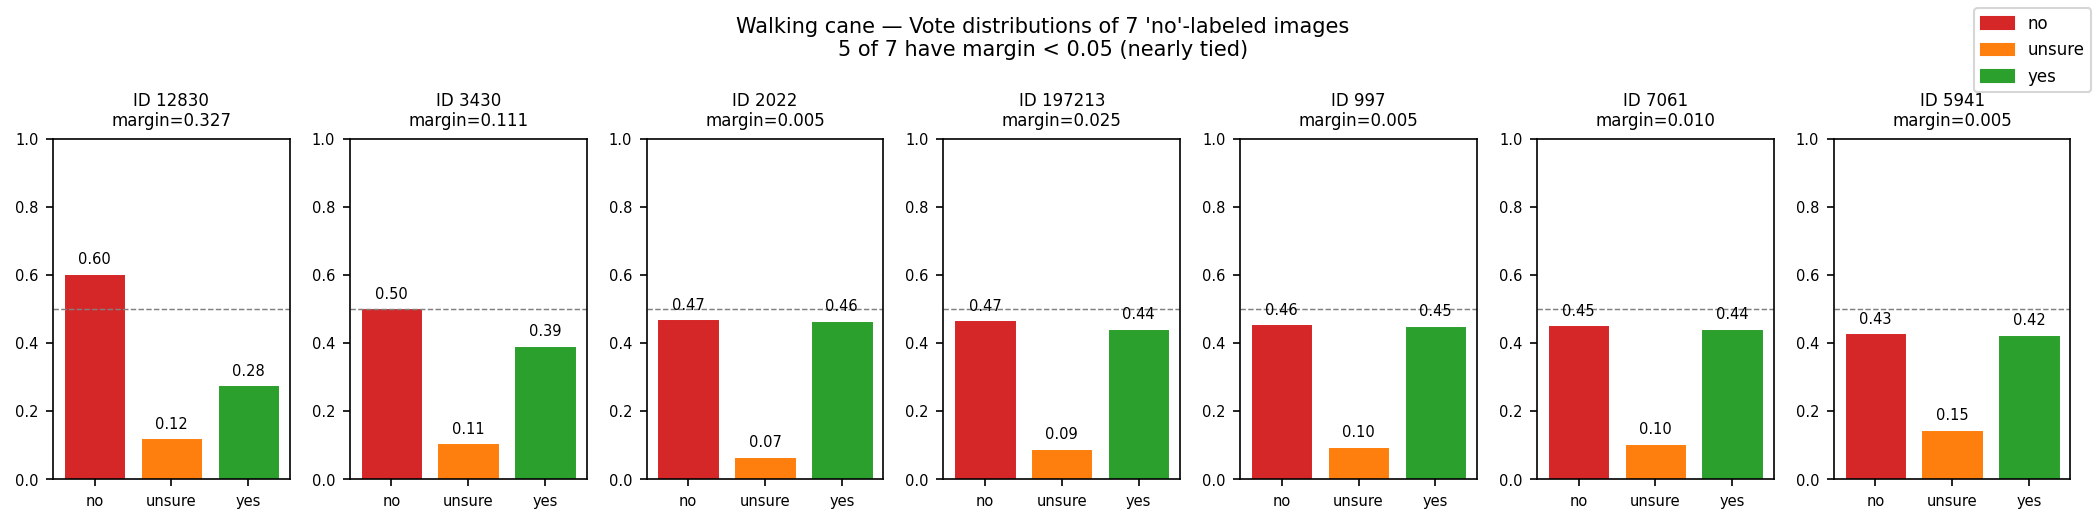
\includegraphics[width=\linewidth]{images/walking_cane_votes.png}
\caption{\textbf{The seven majority-``no'' walking-cane images and their vote distributions.} IDs 2022, 197213, 997, 7061, and 5941 all have margin $<0.05$ between the top two classes (``no'' and ``yes''). Hard-CE training treats these as confident negatives and conflicts with the 45 confident positives in the rest of the cane distribution. Soft-KL retains the empirical bimodality and predicts $[\hat{p}_\mathrm{no} \approx 0.4, \hat{p}_\mathrm{unsure} \approx 0.1, \hat{p}_\mathrm{yes} \approx 0.5]$, the calibrated correct answer.}
\label{fig:supp_failures}
\end{figure*}

\end{document}
